\documentclass[10pt,a5paper,twoside]{book}
\usepackage[utf8]{inputenc}
\usepackage[czech]{babel}
\usepackage[T1]{fontenc}
\usepackage{amsmath}
\usepackage{amsfonts}
\usepackage{amssymb}
\usepackage{hyperref}
\usepackage[dvips]{graphicx}
\usepackage[top=1.5cm, left=1.2cm, bottom=1.2cm, includefoot]{geometry}
\usepackage{eso-pic}
\usepackage{pdfpages}
\usepackage{textpos}
\usepackage{titlesec}
\usepackage{verbatim}
\usepackage{multicol}

\fontencoding{T1}
\fontfamily{cmss}
\fontseries{m}
\fontshape{n}
\setlength{\belowcaptionskip}{-15pt} % mezera za popiskem obrázku
\usepackage{xcolor}
\usepackage{pdfpages}
% pdftk TitlePage14_1.pdf Jihacas14_1.pdf cat output Jihocas_14_1-WEB_kontrola.pdf spojeni pdf

\titleformat{\section}
{\color{black}\normalfont\Large\bfseries}
{\color{black}\thesection}{1.2em}{}

\newcommand{\autor}[1]{
	\begin{flushright}
	\textit{#1}
	\end{flushright}
}

\begin{document} 

%\begin{titlepage}
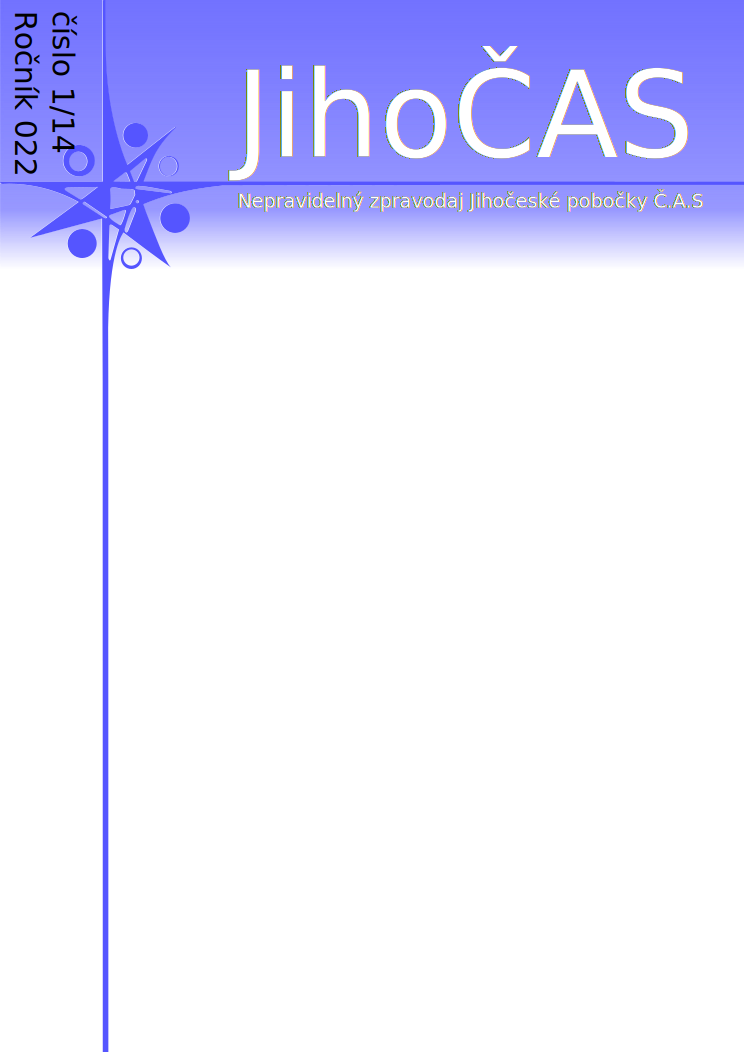
\includepdf{TitlePage.pdf}

\end{titlepage}



\section*{K obrázku na titulní straně}
Fotografie ze stavby hvězdárny Františka Pešty v Sezimově Ústí z roku 1964. Druhá fotografie je novější (1999).
\vfill
\section*{JihoČAS}
Vydává: Jihočeská pobočka České astronomické společnosti.\\
Redakce a adresa pro zasílání příspěvků: Martin Kákona, U Jatek 19/III, 392 01 Soběslav, e-mail: \href{mailto:martin.kakona@astro.cz}{martin.kakona@astro.cz}.\\
Sazba: Roman Dvořák, e-mail: \href{mailto:roman-dvorak@email.cz}{roman-dvorak@email.cz}.\newpage



\section*{Podkarpatská astronomická společnost}
\autor{Petr Bartoš a kol.}

Podkarpatská astronomická společnost byla založena v roce 1928 jako první pobočka České astronomické společnosti. Jejím hlavním úkolem bylo Šíření poznatků z astronomie mezi nejširší veřejností. V roce 1930 se Pešta stává okresním účetním Okresního úřadu v Tačově, což má za následek utlumení jeho astronomických aktivit. Na Podkarpatské Rusi pracuje až do roku 1939, kdy jeho pobyt ukončil vpád maďarských vojsk.


\subsection*{Podkarpatská Rus}

Podkarpatská Rus, jako součást Československé republiky, měla v té době vlastní sněm, který volil předsednictvo. Sněm Podkarpatské Rusi byl příslušný usnášet se o zákonech ve věcech „jazykových, vyučovacích, náboženských, místní správy, jakož i v jiných věcech, které by naň přenesly zákony Československé republiky.“ Zákony přijaté sněmem Podkarpatské Rusi, projevil-li s nimi prezident souhlas svým podpisem, vyhlašovali se ve zvláštní sbírce a podepisoval je také guvernér. 
\par Prvním guvernérem Podkarpatské Rusi byl zvolen Grigorij Žatkovič (26. 4. 1920 - březen 1921), později guvernérskou funkci vykonával Anton Beskid (listopad 1923 - červen 1933) a Konstantin Hrabar (březen 1935 - říjen 1938).
\par Nikdy v dějinách neprožila Podkarpatská Rus takový vzestup jako v letech 1919 - 1939, třebaže státní byrokracie bohužel brzdila rychlejší rozvoj podkarpatské autonomie. Svou "podkarpatskou hru" rozehrála i maďarská vláda, která poslala v říjnu 1921 stížnost společnosti národů, jejímž hlavním názorem bylo, že Československo na Podkarpatsku neplní závazky z mírových smluv. Budapešti se především nelíbilo, že se zemi dosud nedostalo autonomie. Československo vysvětlilo svou politiku na Podkarpatské Rusi i překážky, které se stavěly proti okamžité autonomii, tak přesvědčivě, že Společnost národů československé stanovisko přijala a došla k závěru, že "československá vláda podala přehled práce, již vykonala, aby vychovala lid a uschopila jej k autonomii." Vyslovila však přesvědčení, že Československo "v brzké budoucnosti najde prostředky, jak přikročit k vybudování území Podkarpatské Rusi jako samosprávné jednotky podle mírové smlouvy." 
\par Neblahé dědictví chudoby materiální i duchovní, bída, negramotnost, nemoce, nízká úroveň průmyslové i zemědělské produkce - to všechno podstatně ztěžovalo další cestu. V okolních státech se nastolily polodiktátorské režimy, v nedalekém Sovětském svazu řádil hladomor a krvavá Leninova revoluce vyhlazovala politické odpůrce. Československo a Podkarpatsko však zůstaly ostrovem demokracie a vzestupu. Rozvinul se společenský a politický život dosud v této zemi nevídaný. Připravovaly se podmínky pro autonomii země, v Užhorodě i v jiných městech byly postaveny vládní a správní budovy, které sloužily místním potřebám a v nichž měly začít fungovat sněm i vláda. Otevíraly se nové školy, stavěly silnice a železnice, vznikaly nemocnice. 
\par Bylo by však omylem idealizovat meziválečné poměry na Podkarpatsku. Pozůstatky minulosti byly tak značné, že se je nemohlo podařit při nejlepší vůli zlikvidovat. Vesnicemi obcházely hlad, bída a nemoce, hladové pochody, prosebná procesí i demonstrace trvaly ještě poté, co ochabla největší tíže hospodářské krize konce dvacátých let. To vše se projevovalo i ve volebních preferencích pro komunistickou stranu využívající těchto neblahých poměrů (v celém období první republiky tu patřila k nejsilnějším politickým stranám). Přesto všechno byl lid Podkarpatské Rusi vděčný za to, že mohl žít v rámci ČSR, a proto při oslavách desátého výročí spojení Podkarpatské Rusi s Československem v roce 1929 daroval Praze roubený kostelík sv. Michala z Medvedovců u Mukačeva. Na náklady podkarpatského lidu byl kostelík přenesen na pražský Petřín, kde stojí dodnes.
\par 11. října 1938 byla vytvořena nakrátko autonomní vláda Podkarpatské Rusi v čele s Andrejem Brodym, spjatým s Budapeští pevnými svazky víc, než se slušelo na předsedu autonomní vlády. Současně v dohodě s hitlerovským Německem usilovalo Maďarsko o revizi mírových smluv a návrat k situaci před rokem 1919. Po Brodym následovala 24. října druhá autonomní vláda Augustina Vološina. 
\par Po dvou zákonech o samosprávě Podkarpatské Rusi a o zemském guvernérovi z roku 1937 vyhlásila 22. listopadu 1938 československá vláda konečně autonomii Podkarpatské Rusi zatím zajištěnou formálně v ústavě. Ve vládní vyhlášce se uvedla v činnost podkarpatská vláda a měl být svolán sněm Karpatské Ukrajiny. Týž den byla ustavena i autonomie Slovenska. Senát schválil zákon navržený Národním shromážděním jednomyslně.
\par Jenže již předtím dal Hitler svolat na 2. listopadu 1938 v návaznosti na mnichovský diktát arbitrážní konferenci do Vídně. Podle jejího rozhodnutí muselo Československo odevzdat Maďarsku jižní část Slovenska a jih Podkarpatské Rusi s Užhorodem, Mukačevem a Berehovem. Maďaři zabrali 152 tisíc hektarů nejúrodnější části země s vinicemi, ovocnými sady, tabákovými a kukuřičnými plantážemi. Přerušili tak hlavní železniční trať od Čopu na východ. Hlavním městem země se stal Chust, kde kněz a spisovatel Augustin Vološin ustanovil autonomní vládu Karpatské Ukrajiny.  
\newpage
\begin{figure}[!htbp]
 \centering
  \includegraphics*[width=12cm]{mapa.jpg}
\end{figure}

Výřez z mapy Československa z roku 1935, v kroužku je zvýrazněn \\Užhorod. 

\subsection*{Založení Podkarpatské astronomické společnosti v Užhorodě}
\par Podkarpatská astronomická společnost v Užhorodě byla ustavena dne 30. března 1928, a to jako odbočka České astronomické společnosti v Praze. Zásluhou tehdejšího jednatele Františka Pešty, úředníka zemského úřadu v Užhorodě byly překonány veškeré nesnáze, které stály v cestě založení společnosti. František Pešta byl v kontaktu s jednatelem České astronomické společnosti panem Klepeštou, jemuž v několika dopisech popsal, jak došlo k založení společnosti. V další korespondenci podal zprávu o výsledku prvních schůzek a rovněž odpověděl na dotaz, jak hodlá společnost uvést v život. Pešta tehdy prohlásil, že budou pořádány přednášky, k nimž má již vypracované podklady, a které postupně uveřejňuje v jediném českém deníku vycházejícím na Podkarpatské Rusi, v Podkarpatských Hlasech. Zároveň informoval o připravovaných vycházkách s dalekohledem, při nichž budou členové seznamováni s hvězdnou oblohou a vycházky by pak doplňoval výkladem teoretického hvězdářství. 
\par I když stanovy České astronomické společnosti umožňovaly vznik místních poboček a sekcí, tehdy nazývaných místními odbory, neměl nikdo ve společnosti s tímto zkušenosti. Proto pan Pešta na svůj dotaz, jak docíliti založení místního spolku, obdržel poměrně nekonkrétní odpověď s tím, že podobný dotaz již obdrželi i z Brna. Výbor společnosti tak poradil, aby podali prozatím přihlášku, kterou posoudí Valná hromada České astronomické společnosti a do doby než bude rozhodnuto jinak, nechť se scházejí jako volné sdružení bez vyřizování formalit a hlášení policii. To vše si dal za cíl projednat výbor společnosti „než bude přikročeno k ustavení jednotlivých odborů na venkově.“


\begin{figure}[!htbp]
 \centering
  \includegraphics*[width=12cm]{dum.jpg}
\end{figure}
Budova oblastní rady v Užhorodě, postavená ve 30. letech 20. století\\

\par Rady o fungování spolku obdržely v Užhorodě s povděkem, ovšem odlišnost právních úprav života na Zakarpatské Rusi od právních úprav v zemích historických si vyžádala založení spolku. Stanovy byly připraveny podle vzoru stanov České astronomické společnosti, pouze s nezbytnými drobnými odchylkami, které si vyžádaly místní poměry. Již před registrací spolku, se tento hlásil k úzké spolupráci s Českou astronomickou společností, a to dokonce tak úzké, že byla přímo deklarována ve stanovách spolku. Před registrací spolku byly stanovy rovněž konzultovány s výborem společnosti.
\par Na několika schůzích před samotným založením spolku byly kromě projednání stanov rovněž diskutovány otázky pořízení dalekohledu, vybavení knihovny a pronájem vhodných prostor pro konání schůzek. Z počátku se schůze konaly v prostorách Methodistické církve, za což ji výbor spolku vřele poděkoval.
\par Na základě předložené žádosti ze dne 6. 4. 1928 doplněné o stanovy, byly stanovy Podkarpatské astronomické společnosti v Užhorodě schváleny Civilní správou Podkarpatské Rusi, a to dne 7. 5.1928. Následně si ověřenou kopii stanov vyžádalo Finanční ředitelství v Užhorodě. Podmínkou činnosti bylo hlášení konání každé valné hromady Policejnímu ředitelství v Užhorodě a podávání zpráv o jejím výsledku, případně o změnách u jednotlivých funkcionářů tamtéž.

\subsubsection*{Spolupráce s Českou astronomickou společností}
\par Na základě vzájemné dohody s Českou astronomickou společností byl každý člen Podkarpatské astronomické společnosti v Užhorodě zároveň členem České astronomické společnosti v Praze. Členský příspěvek byl stanoven ve výši 20 Kč ročně, z kterého byla polovina odváděna ČAS v Praze. Předplatné časopisu Říše hvězd činilo v roce 1928 15 Kč ročně, odznak a legitimace pak 6 Kč. Předsedou Podkarpatské astronomické společnosti v Užhorodě se stal Dr. Rudolf Kyzlík, místopředsedou Dr. Ivan Kossey, jednatelem František Pešta a pokladníkem Štěpán Smutný. Mezi další body dohody patřilo i umožnění zveřejňování informací v Říši hvězd. Oficiálně byla vzájemná spolupráce popsána v paragrafu 16, stanov Podkarpatské astronomické společnosti v Užhorodě:
\par Podkarpatská astronomická společnost jest přičleněna k České astronomické společnosti v Praze, s níž se dohodne o spolupráci a v dohodě s touto bude též pracovati o zakládání poboček na Podkarpatské Rusi. České astronomické společnosti budou pravidelně půlletně podávány zprávy o činnosti společnosti užhorodské. Každý člen Podkarpatské astronomické společnosti bude zároveň členem České astronomické společnosti dle dohody, kterou výbor s touto společností uzavře. Podrobné propracování spolupráce s Českou astronomickou společností přísluší správnímu výboru, který o tom podá valné hromadě zvláštní zprávu. Právo členů Podkarpatské astronomické společnosti býti členy České astronomické společnosti nijak nepřekáží tomu, aby mohli býti se souhlasem výboru členy i jiných astronomických společností, jsou však povinni pečovati v prvé řadě o rozkvět české vědy astronomické a o rozvoj spolku. 
    \newpage

\subsection*{Činnost Podkarpatské astronomické společnosti}
\par První valná hromada Podkarpatské astronomické společnosti se uskutečnila krátce po registraci stanov v roce 1928. Na této valné hromadě byly stanoveny základní úkoly společnosti a byl nastíněn program společnosti na nejbližší období.

\subsubsection*{První rok (1928-1929)}
\par Podkarpatská astronomická společnost měla svoji druhou valnou hromadu po prvním roce fungování 24. května 1929. Podle jednatelské zprávy bylo konáno v prvním roce činnosti společnosti 5 schůzí s přednáškami Františka Pešty na téma: názory na tvar Země, o vzniku dne a noci, o vzniku fází Měsíce, o zdánlivém pohybu Slunce a o souhvězdích. Vedle toho uspořádala astronomická společnost v tělocvičně Sokola v Užhorodě přednášku o poměru Země k Vesmíru. Astronomie byla v té době také hojně propagována tiskem, kdy např. v Podkarpatských Hlasech uveřejnil František Pešta 38 populárních článků z astronomie. 
\par Astronomická společnost rovněž požádala školní odbor Zemského úřadu Podkarpatské Rusi o zakoupení Zeissova dalekohledu Asegur, ale do doby konání valné hromady neobdržela odpověď. Proto pokračovalo pozorování menším dalekohledem o průměru 70 mm, který společnosti zapůjčil tehdejší guvernér Podkarpatské Rusi Dr. Anton Beskid. 
\par Pravidelné schůzky Podkarpatské astronomické společnosti se konaly v prostorách Methodistického sboru, jehož představenstvo nepožadovalo žádnou úhradu, pouze dobrovolný drobný příspěvek na osvětlení.
\par Pod vedením Františka Pešty se uskutečnilo v měsících březnu, dubnu a květnu celkem 20 pozorování za účasti 170 osob. Byly pozorovány planety Saturn, Merkur, Venuše dále Měsíc, hvězdokupy, dvojhvězdy a sluneční skvrny. 
\par Ke konci roku 1928 měla Podkarpatská astronomická společnost 15 řádných členů. Výběr členských příspěvků se v roce 1928 protáhl díky dvěma, nám neznámým, členům až do počátku listopadu, i když původní termín měl být již v září. Julius Huska, který původně projevil zájem o členství, se tohoto nakonec vzdal, protože při velkém zadlužení na stavbu domu mu již nezbývaly prostředky pro zaplacení členských příspěvků. 
\par V srpnu 1928 byl spolek vyzván k připojení se k oslavám 10. výročí vzniku Československé republiky. V rámci oslav byly nabízeny možnosti zúčastnit se kulturního programu, vytvoření alegorického vozu a dále byl vyzván zda má sám nějakou jinou představu o účasti k výročí. V archivních materiálech se bohužel informace o účasti spolku na oslavách nedochovala.

\subsubsection*{Druhý rok (1929-1930)}
\par Druhý rok existence Podkarpatské astronomické společnosti byl rokem částečného zklamání, protože část členů byla přeložena na úřady zpět do Čech. 
\par V roce 1930 odjel František Pešta na dovolenou do Čech. Při té příležitosti neopomenul navštívit Prahu a především petřínskou hvězdárnu. Peštovi se zalíbil lustr ve tvaru Saturnu, který viděl v zasedací místnosti petřínské hvězdárny. Poslal tedy dotaz kde a za kolik je možné jej opatřit a tím se z korespondence dozvídáme, že takový lustr v té době stál 70,- Kč, co je ale zajímavější, že Pešta obýval byt (garsonku) o rozměrech 5x3x3 metry, což rozhodně není mnoho.
\par Pod vedením Františka Pešty se opět uskutečnilo pozorování planet Jupiter, Saturn, Mars, Venuše dále Měsíc, hvězdokup, dvojhvězd a slunečních skvrn. Pro velký zájem veřejnosti o pozorování měsíčního povrchu bylo za příznivého počasí rozšířeno pozorování téměř na celý týden.
\par Zajímavou zmínkou vyplývající ze zachovalé korespondence je schvalování valných hromad policejním ředitelstvím. Na závěr každého schválení je poznámka: „Za přesné dodržení schváleného programu a zákonný průběh této schůze činím svolavatele, resp. předsednictvo osobně zodpovědnými.“ 

\subsubsection*{Kritický rok 1930}
\par První polovina roku 1930 probíhala celkem bez větších problémů a nic nenaznačovalo tomu co má přijít. V březnu zaslal spolek blahopřejný dopis k 80. narozeninám prezidenta Československé republiky. Za blahopřání obdržel spolek poděkování prezidentské kanceláře podepsané zemským prezidentem. 
\par Po návratu z Čech se Pešta začátkem září 1930 dozvídá, že bude ještě s několika dalšími mladými úředníky přeložen z Užhorodu do okresního města. 
\par Na základě dopisu Klepešty a Nušla z České astronomické společnosti nedošlo k přeložení Fr. Pešty s ostatními úředníky do okresů. Ten pln nového nadšení vyhlásil na podzim roku 1930 celkem 5 přednášek v dělnické akademii a další rozjednal s klubem turistů. Pravdou je, že účast pouhých pěti posluchačů na první přednášce, byla zklamáním, ale hned na následující přednášku se dostavilo 50 posluchačů. 25. listopad 1930 je ovšem studenou sprchou. Pešta okamžitě píše do Prahy o svém přeložení do okresu Ťačovo, které by mělo nastat již 1. prosince 1930. 
\par Ještě koncem listopadu 1930 předává Pešta agendu Podkarpatoruské astronomické společnosti v Užhorodě Dr. Kyzlíkovi a pokladnu panu Smutnému. Protože Kyzlík ani Smutný nejeví přílišnou aktivitu ve správě spolku, předpokládá Pešta jeho brzký zánik. Protože nové místo působnosti Pešty je 150 km od Užhorodu, vystupuje z Podkarpatoruské astronomické společnosti a hlásí se zpět za přímého člena České astronomické společnosti. 

\subsubsection*{Rok 1931 – konec Podkarpatské astronomické společnosti}
\par Na řádnou valnou hromadu, konanou 13. listopadu 1931 v restauraci „Kvasná voda“ se dostavili pouze čtyři členové spolku. Hlavním bodem jednání valné hromady byla další existence Podkarpatské astronomické společnosti, která byla odchodem Františka Pešty do Ťačova (foto Ťačova z roku 2001) téměř zcela ochromena. Za rok trvající popsané situace se nepodařilo najít nikoho, kdo by převzal po Peštovi odbornou stránku fungování spolku. 
\par Po dlouhé diskuzi bylo rozhodnuto o ukončení činnosti a likvidaci spolku. Likvidací po stránce právní byl pověřen předseda Podkarpatské astronomické společnosti Dr. Rudolf Kyzlík, likvidací po stránce finanční byl pověřen pan Radocha. V rámci ukončení činnosti bylo rozhodnuto, že nevybrané členské příspěvky byly odepsány, protože v roce 1930 a 1931 společnost nevyvíjela prakticky žádnou činnost. Příspěvky zaplacené v roce 1930 byly použity pro uhrazení časopis a s účetním zůstatkem bylo naloženo dle stanov. 
\par Na závěr valné hromady byl vysloven dík Františku Peštovi za jeho vykonanou práci. Z dopisu pana Radocha o ukončení činnosti, adresovaném České astronomické společnosti, je zajímavý výrok: „Je sice dosti smutné, že došlo v místě k těmto koncům, ale muselo to být, neboť byli bychom úředně rozpuštěni, ježto spolek odchodem pana Pešty usnul spánkem tvrdým.“
\par Likvidace Podkarpatské astronomické společnosti proběhla na přelomu roku 1931 a 1932. Česká astronomická společnost převzala účetní zůstatek a listinné materiály k archivaci v únoru 1932. V témže období bylo ukončení činnosti oznámeno úřadům v Užhorodě.
\par Z Prahy obdrželi členové spolku ještě dopis od Klepešty a Nušla, ve kterém jsou vyzíváni, aby v případě svého pokračujícího zájmu o astronomii nevystupovali z České astronomické společnosti.
\par Jako nádherné zhodnocení činnosti spolku uvádím zde úryvek z dopisu pana Radocha, adresovaném České astronomické společnosti: „Pokud jde o mou osobu nevím jak se rozhodnout, neboť byť jsem časopisu příliš nerozuměl, což je pro mne neklamnou známkou, že astronom ze mne asi nebude, přece příliš rád si vzpomenu na to, že dík vašim atlasům a mapám stala se mně obloha místem, kam vždy rád pohlédnu a mé večerní procházky byly obohaceny o nový velký prožitek.“
\newpage
\subsection*{Členové Podkarpatské astronomické společnosti}

\begin{tabular}{l l p{5.5cm}}
\textbf{Jméno, příjmení}& \textbf{členství} & \textbf{poznámky (funkce, odběr Říše hvězd, zaměstnání, ...)} \\
\hline\hline
Dr. Rudolf Kyzlík				&1928-1929&	předseda\\
Ing. František Homolka	&1928-1929&	člen výboru, Říše Hvězd, lesní referent, přestoupil do Čech\\
Štěpán Smutný					&1928-1929&	pokladník, Říše Hvězd, účetní tajemník civilní správy v Užhorodě\\
Leopold Hlavatý				&1928-1929&	revizor účtu, Říše Hvězd, účetní tajemník civilní správy v Užhorodě\\
Ladislav Rajtr					&1928-1930&	Říše Hvězd, účetní adjunkt civilní správy v Užhorodě, přeložen\\
Antonín Radocha				&1928-1930&	knihovník, Říše Hvězd, účetní adjunkt civilní správy v Užhorodě\\
František Pešta					&1928-1930&	jednatel, Říše Hvězd, účetní elév civilní správy v Užhorodě\\
Ing. Josef Zajíc					&1928-1929&	Říše Hvězd, tajemník Republikánské strany\\
Marie Janoušková				&1928	&člen výboru, choť bankovního úředníka, přestoupila do Čech\\
Emanuel Janoušek			&1928-1929&	revizor účtu, Říše Hvězd, úředník Slovenské banky\\
Dr. Ivan Kosej					&1928-1929&	místopředseda, Říše Hvězd\\
Josefa Turečková				&1928-1929&	člen výboru, Říše Hvězd, přestoupila do Čech\\
Josef Vrbec							&1928	&Říše Hvězd, účetní adjunkt civilní správy v Užhorodě, přeložen\\
Dr. Otto Pavluch				&1930	&Říše Hvězd\\
Josef Pumpr						&1930	&Říše Hvězd\\
Ing. Oldřich Kadeřábek	&1928&\\
Julius Hustka						&(1928)&	civilní správa v Užhorodě\\
\end{tabular}
\newpage



\subsection*{Hospodaření Podkarpatské astronomické společnosti}


\subsubsection*{Hospodaření v roce 1928}
\begin{tabular}{p{9cm} r}
Příjmy za rok 1928	&433,- Kč\\
Výdaje za rok 1928	&398,- Kč\\
$\;$    z toho odvody do Prahy (ČAS)	&314,- Kč\\
$\;$    z toho kolky	  &44,- Kč\\
$\;$    z toho dávka za úřední výkon	  &30,- Kč\\
$\;$    z toho poštovné	  &10,- Kč\\
Zůstatek ke konci roku 1928	  &35,- Kč\\
\end{tabular}
\\
\subsubsection*{Hospodaření v roce 1929}
\begin{tabular}{p{9cm} r}
Převod z roku 1928	  &35,- Kč\\
Příjmy za rok 1929	&400,- Kč\\
Výdaje za rok 1929	&280,- Kč\\
$\;$    z toho odvody do Prahy (ČAS)	&280,- Kč\\
Zůstatek ke konci roku 1929&	155,- Kč\\
\end{tabular}
\\
\subsubsection*{Hospodaření v roce 1930}
\begin{tabular}{p{9cm} r}
Převod z roku 1929	&155,- Kč\\
Příjmy za rok 1930	   & 0,- Kč\\
Výdaje za rok 1930	    &0,- Kč\\
Zůstatek ke konci roku 1930	&155,- Kč\\
\end{tabular}
\\
\subsubsection*{Hospodaření v roce 1931}
\begin{tabular}{p{9cm} r}
Převod z roku 1930	&155,- Kč\\
Příjmy za rok 1931	&119,- Kč\\
Výdaje za rok 1931	    &0,- Kč\\
$\;$    z toho odvody do Prahy (ČAS)	    &0,- Kč\\
Zůstatek ke konci roku 1931	&274,- Kč\\
\end{tabular}

\newpage
\section*{50 let Hvězdárny Fr. Pešty v Sezimově Ústí \\se blíží}
V roce 2015 oslaví hvězdárna v Sezimově Ústí již 50. výročí svého otevření. Hvězdárna byla založena Františkem Peštou, po kterém byla později také pojmenována. V současné době připravují členové hvězdárny oslavy, jejichž hlavní část proběhne v říjnu tohoto roku. Protože však došlo k otevření 6.6.1965, i na toto datum připadne jedna slavnostní oslavička, a to 6.6.2015 od 13 hodin proběhne v prostorách hvězdárny setkání všech členů a pamětníků. Srdečně proto zveme všechny, kteří se podíleli na činnosti hvězdárny v Sezimově Ústí, aby přišli do částečně zrekonstruované a přistavěné hvězdárny nejen zavzpomínat. Setkání bude také poslední příležitostí, jak přispět do připravované publikace o historii hvězdárny a astronomie v Sezimově Ústí.
Při této příležitosti probíhá již zmiňovaná přístavba, rekonstrukce a různé opravy, které zapříčinily i nutnost důkladného úklidu. Nabízíme proto za odvoz desítky starších astronomických publikací převážně v ruštině a němčině, případně publikace, které máme ve více výtiscích.
Vše o oslavách, rekonstrukci apod. můžete nalézt rovněž na webu hvězdárny:  www.hvezdarna-fp.eu

\section*{Kresba Měsíce, sladěná s hlavním tématem…}
\autor{Milan Blažek,\\
 Hvězdárna a planetárium hl. m. Prahy, p. o.}

Vážení čtenáři JihoČASu, původně jsem měl připraven jiný příspěvek, avšak v okamžiku, kdy jsem se dověděl, že tento JČ bude nejen černobílý, ale hlavně historicky zaměřený, rozhodl jsem se i já tomu přizpůsobit… Snad můj příspěvek alespoň trochu tematicky zapadne do rázu tohoto vydání.
Předkládám tedy jednu (z mého pohledu již téměř historickou) kresbu Měsíce, na které je zachycen náš vesmírný soused v období kolem první čtvrti.
Kresba byla pořízena před patnácti lety, při pozorování malým čočkovým dalekohledem o průměru objektivu 60mm, zvětšení 47$\times$. Dalekohled poskytoval pochopitelně převrácený obraz, kresba je však překreslena v orientaci sever nahoře, východ vpravo, aby korespondovala s tím, jak vidíme jeho siluetu při pohledu prostým zrakem.


%\begin{figure}[htbp]
% \centering
%  \includegraphics*[width=10cm]{moon.jpg}
%\end{figure}
%\begin{figure}[htbp]
% \centering
%  \includegraphics*[width=10cm]{JH/moon.eps}
%\end{figure}




\end{document}
 
 
%	\begin{itemize}
%	\item 
%	\end{itemize}
